\documentclass[../../main.tex]{subfiles}

\begin{document}
\section{Binary Tree Tensor Networks}
    We are interested in the model space of binary tree tensor networks as shown in figure~\ref{fig:binary_tree_tensor_network}. We assume that every network is non-negative and normalized, and we set $f \equiv \text{id}$ (see appendix~\ref{section:tensor_networks}).

    \begin{figure}[h]
        \centering
        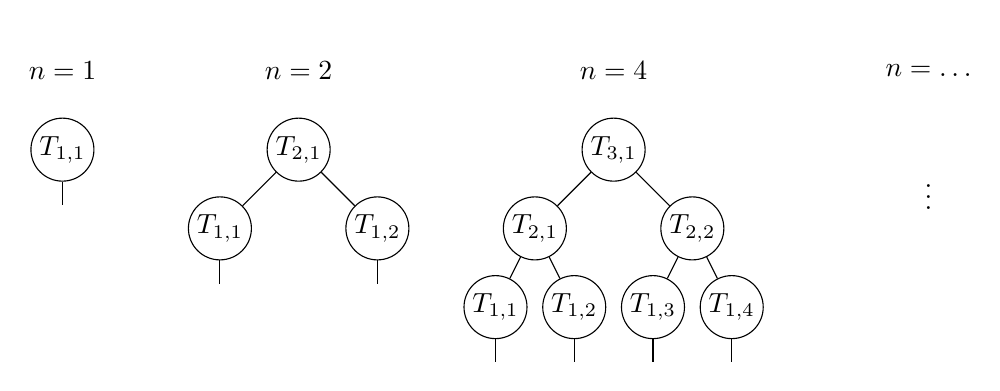
\begin{tikzpicture}[
            every node/.style={circle, draw, minimum size=8mm, inner sep=0pt},
            level distance=10mm,
            sibling distance=10mm,
            edge from parent/.style={draw},
            level 1/.style={sibling distance=20mm},
            level 2/.style={sibling distance=10mm}
        ]

        % Tree with 1 leaf
        \node[draw=none] at (-6,0) {$n=1$};
        \node (t11a) at (-6,-1) {$T_{1,1}$};
        \draw (t11a) -- ++(0,-0.7);

        % Tree with 2 leaves
        \node[draw=none] at (-3,0) {$n=2$};
        \node (t21) at (-3, -1) {$T_{2,1}$} [grow=down]
        child {node (t11b) {$T_{1,1}$}}
        child {node (t12) {$T_{1,2}$}};
        \draw (t11b) -- ++(0,-0.7);
        \draw (t12) -- ++(0,-0.7);

        % Tree with 4 leaves
        \node[draw=none] at (1,0) {$n=4$};
        \node (t31) at (1, -1) {$T_{3,1}$} [grow=down]
        child {node (t21a) {$T_{2,1}$}
            child {node (t11c) {$T_{1,1}$}}
            child {node (t13) {$T_{1,2}$}}}
        child {node (t22) {$T_{2,2}$}
            child {node (t14) {$T_{1,3}$}}
            child {node (t15) {$T_{1,4}$}}};
        \draw (t11c) -- ++(0,-0.7);
        \draw (t13) -- ++(0,-0.7);
        \draw (t14) -- ++(0,-0.7);
        \draw (t15) -- ++(0,-0.7);

        % Dots representing omitted trees
        \node[draw=none] at (5,0) {$n=\dots$};
        \node[draw=none] at (5,-1.5) {$\vdots$};
        \end{tikzpicture}
        \caption{Binary tree model space for sequences of length $n = 2^k$.}
        \label{fig:binary_tree_tensor_network}
    \end{figure}

\subsection{Bulk Marginal Property}
    In definition~\ref{def:induced_bulk_marginal_model} we saw how to construct a model with the desired bulk marginal property based on the base model. However, we might not always have a base model for every $n \in \mathbb{N}$ like discussed. Luckily, it turns out that this is not an issue, as there are many ways we can build a new model with the bulk marginal property from a base model even if it is only defined on a subset of $\mathbb{N}$. Without a proof, we might do the same procedure as in definition~\ref{def:induced_bulk_marginal_model} but with bigger steps (instead of taking always the consecutive model), and induce the in-between models by marginalizing the bigger ones.

    Alternatively, if we wanted a model with bulk marginal property that itself is also an element of our specified model space, we might ask ourselves, how we can construct a bigger tensor network while preserving the distribution in its leading random variables.

    Let's analyze the following example: Say we wanted to integrate the tree tensor network for $n = 2$ in figure~\ref{fig:binary_tree_tensor_network} into a bigger tree tensor network with $n = 4$. Note that by assumptions the tensor networks are non-negative and normalized, and $f \equiv \text{id}$. Based on proposition~\ref{proposition:marginalized_tensor_network}, it follows that in order for our new tensor network to have the bulk marginal property, contracting the smaller network must be equivalent to contracting the bigger one, where the new nodes (in this case $T'_{1,3}$ and $T'_{1,4}$) are contracted with all-ones vectors, see figure~\ref{fig:bmp_model_equiv}.

    \begin{figure}[h]
        \centering
        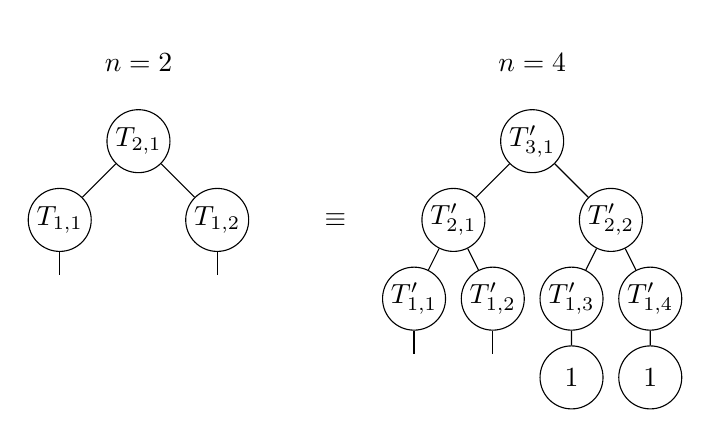
\begin{tikzpicture}[
            every node/.style={circle, draw, minimum size=8mm, inner sep=0pt},
            level distance=10mm,
            sibling distance=10mm,
            edge from parent/.style={draw},
            level 1/.style={sibling distance=20mm},
            level 2/.style={sibling distance=10mm}
        ]
            \node [draw=none] at (-5,0) {$n=2$};
            \node (t21) at (-5, -1) {$T_{2,1}$} [grow=down]
            child {node (t11b) {$T_{1,1}$}}
            child {node (t12) {$T_{1,2}$}};
            \draw (t11b) -- ++(0,-0.7);
            \draw (t12) -- ++(0,-0.7);

            \node [draw=none] (eqv) at (-2.5, -2) {$\equiv$};

            \node[draw=none] at (0,0) {$n=4$};
            \node (t31) at (0, -1) {$T'_{3,1}$} [grow=down]
            child {node (t21a) {$T'_{2,1}$}
                child {node (t11c) {$T'_{1,1}$}}
                child {node (t13) {$T'_{1,2}$}}}
            child {node (t22) {$T'_{2,2}$}
                child {node (t14) {$T'_{1,3}$}
                    child {node {$\bm{1}$}}}
                child {node (t15) {$T'_{1,4}$}
                    child {node {$\bm{1}$}}}};
            \draw (t11c) -- ++(0,-0.7);
            \draw (t13) -- ++(0,-0.7);
        \end{tikzpicture}
        \caption{Bulk marginal property enforces the equivalence of these models.}
        \label{fig:bmp_model_equiv}
    \end{figure}

    Note that if we indeed had equivalence of these models, this would imply that the bigger model is now normalized as well based on lemma~\ref{lemma:normalized_tensor_networks}.

    Let's now analyze the vector $\bm{v}$ depicted in figure~\ref{fig:sufficient_condition_bmp}.

    \begin{figure}[h]
        \centering
        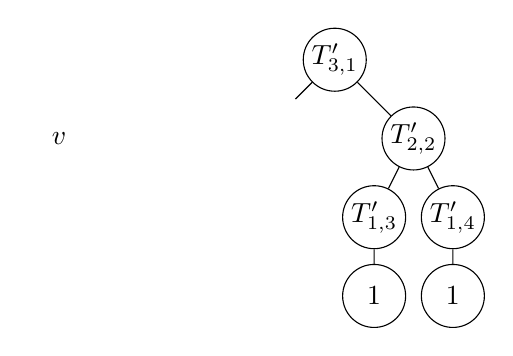
\begin{tikzpicture}[
            every node/.style={circle, draw, minimum size=8mm, inner sep=0pt},
            level distance=10mm,
            sibling distance=10mm,
            edge from parent/.style={draw},
            level 1/.style={sibling distance=20mm},
            level 2/.style={sibling distance=20mm}
        ]
            \node [draw=none] (v) at (-4, -2) {$\bm{v}$};

            \node [draw=none] (eqv) at (-2.5, -2) {$\coloneqq$};

            \node (t31) at (-0.5, -1) {$T'_{3,1}$} [grow=down]
            child {node (t22) [xshift=1cm] {$T'_{2,2}$}
                child {node (t14) [xshift=0.5cm] {$T'_{1,3}$}
                    child {node (11) {$\bm{1}$}}}
                child {node (t15) [xshift=-0.5cm] {$T'_{1,4}$}
                    child {node (12) {$\bm{1}$}}}};
            \draw (t31) -- ++(-0.5,-0.5);
        \end{tikzpicture}
        \caption{Contracting this sub-network with all-ones vectors yields vector $\bm{v}$.}
        \label{fig:sufficient_condition_bmp}
    \end{figure}

    What can we say about $\bm{v}$? Well, we can assume that it has at least one non-zero entry. This is always possible, and if $\bm{v}$ consisted of only zeros, then the network wouldn't be normalized.

    But now we can initialize the remaining tensors: The leaf tensors $T'_{1,1}$ and $T'_{2,1}$ can be taking over from the smaller model, and the new tensor $T'_{2, 1}$, which is now a vector of matrices like the old $T_{2, 1}$, can initialized as the matrix $T_{2, 1}$ divided by the non-zero entry of $\bm{v}$ at the same position. All other matrices in this vector will just be set to zero-matrices.

    It is apparent that this initialization ensures the equivalence of the models as depicted in figure~\ref{fig:bmp_model_equiv}. It is also clear that this method works when transitioning from any $n = 2^k$ to $n' = 2^{k+1}$. Note that we also didn't increase the sizes of the tensors (except for $T'_{2, 1}$, as it got another axis). Furthermore, when assuming all tensor entries are non-negative, then the new tensor network $\mathcal{T}'$ is also non-negative. This leads to the following observation:

    \begin{corollary}
        Let $\mathcal{T}$ be a binary tree tensor network over $\Sigma^n, n = 2^k$. Then, there exists a binary tree tensor network $\mathcal{T}'$ over $\Sigma^{n'}, n' = 2^{k+1}$ s.t. the transition from $\mathcal{T}$ to $\mathcal{T}'$ complies with the bulk marginal property. Furthermore, $\mathcal{T}'$ complies with axes sizes constrains (under the assumption of a maximum axis size constrain which is increasing in $n$).
    \end{corollary}

\subsection{Binary Tree Tensor Networks are Universal Approximators}
    Now, we want to analyze the properties of these binary tree tensor networks further. It may not bother us how we construct increasingly bigger models that satisfy the bulk marginal property, we know that the model space of binary tree tensor networks is capable of producing such families.

    One question we might ask is whether such a model space restricts the space of possible probability distributions, and if so by how much. As it turns out, in the most general case when allowing very large tensors in the networks, we can model \emph{any} probability distribution:

    \begin{theorem}
        \label{theorem:bttn_are_universal_approximators}
        Given any probability distribution $p: \Sigma^{2^k} \mapsto [0,1]$, we can always construct a binary tree tensor network $\mathcal{T}$ over $\Sigma^{2^k}$ s.t. $p \equiv S_{2^k, \mathcal{T}}$. (Where $\mathcal{T}$ has the properties mentioned in the beginning and axes sizes of $|\Sigma|^{\frac{n}{2}}$ are allowed.)
    \end{theorem}
    \vspace{-2.5em}
    \begin{proof}
        For clarity reasons, we only show how to construct $\mathcal{T}$ for $n = 2^k = 4$. The procedure can easily be extended to the general case.

        Our model structure is depicted in figure~\ref{fig:binary_tree_tensor_network_n_equals_four}.

        \begin{figure}[h]
        \centering
        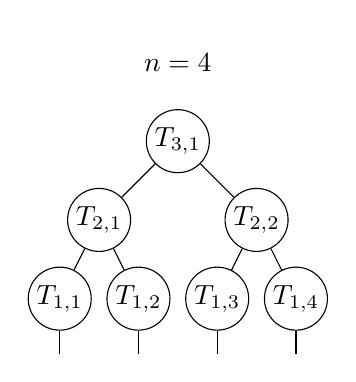
\begin{tikzpicture}[
            every node/.style={circle, draw, minimum size=8mm, inner sep=0pt},
            level distance=10mm,
            sibling distance=10mm,
            edge from parent/.style={draw},
            level 1/.style={sibling distance=20mm},
            level 2/.style={sibling distance=10mm}
        ]

        % Tree with 4 leaves
        \node[draw=none] at (1,0) {$n=4$};
        \node (t31) at (1, -1) {$T_{3,1}$} [grow=down]
        child {node (t21a) {$T_{2,1}$}
            child {node (t11c) {$T_{1,1}$}}
            child {node (t13) {$T_{1,2}$}}}
        child {node (t22) {$T_{2,2}$}
            child {node (t14) {$T_{1,3}$}}
            child {node (t15) {$T_{1,4}$}}};
        \draw (t11c) -- ++(0,-0.7);
        \draw (t13) -- ++(0,-0.7);
        \draw (t14) -- ++(0,-0.7);
        \draw (t15) -- ++(0,-0.7);

        \end{tikzpicture}
        \caption{Model structure of binary tree tensor networks for $n = 2^k = 4$.}
        \label{fig:binary_tree_tensor_network_n_equals_four}
    \end{figure}

    Now, we initialize the leaf matrices as identity matrices $\delta_2 \in \mathbb{R}^{|\Sigma| \times |\Sigma|}$. Thus, when contracting a leaf tensor with a one-hot encoded input vector at position $i$, we get the vector $\bm{v}^{(i)}$ with $\bm{v}^{(i)}_j = \bm{1}[X_i = c_j], c_j \in \Sigma$.

    Now, the tensors in layer two are of the following form:
    \[
    T_{2, j}: |\Sigma| \times |\Sigma| \mapsto \mathbb{R}^{|\Sigma|^2} \quad .
    \]

    \pagebreak
    
    The outgoing axis may be index by $(X'_i, X'_{i + 1}) \in \Sigma^2$. The map is then defined by
    \[
        T_{2, j}(X_i, X_{i + 1}) = \bm{1}[(X'_i, X'_{i + 1}) = (X_i, X_{i + 1})] \quad ,
    \]
    i.e. $T_{2, j}$ is a three dimensional tensor with $|\Sigma| \times |\Sigma|$ many vectors of size $|\Sigma|^2$ which are one-hot encoded vectors of 2-tuples of $\Sigma^2$.

    Finally, $T_{3, 1}$ stores the entire probability distribution:
    \[
        T_{3, 1}: \mathbb{R}^{|\Sigma|^2} \times \mathbb{R}^{|\Sigma|^2} \mapsto [0, 1], ((X'_1, X'_2), (X'_3, X'_4)) \mapsto p(X'_1, X'_2, X'_3, X'_4) \quad .
    \]
    Thus, based on the construction we see that upon contracting the network with an initialization defined by $w \in \Sigma^4$, we get $S_{4, \mathcal{T}}(w) = p(w)$ as desired.

    Note that this construction can easily be extended to arbitrary $n = 2^k$.
    \end{proof}

    As one might expect, we see that our general construction needs $\Omega(|\Sigma|^n)$ many parameters, as the root tensor stores all the $|\Sigma|^n$ many probabilities for $w \in \Sigma^n$.
    % Of course, there cannot be a general model capable of any probability distribution with $o(|\Sigma|^n)$ many parameters.

\subsection{Restricting Parameters}
    One natural question is what happens if we restrict the number of parameters. Intuitively, if we don't have exponentially many parameters with respect to the word length, we won't be able to construct \emph{every} probability distribution.

    However, when modelling natural language for example, we really aren't interested in the most general case of probability distributions.
    For example, we are interested in specific subset of models with power-law behavior.
    % For example, for a fixed word length $n$, we might want behavior similar to large scale time invariance (see definition~\ref{definition:large_scale_time_invariance}).
    Moreover, note that for a fixed $n$, the constraint of the bulk marginal property has no restrictive effect on the space of possible probability distributions.

    % Most decisively,  Our goal is to show that binary tree tensor networks are incapable of this when we cap the number of parameters (i.e. the tensor sizes).

    Let's formalize what it means to cap the parameters. There are two approaches that come to my mind: Either cap the total number of parameters (the entries of \emph{all} tensors), or cap the axes sizes and hence the size of each tensor individually. Of course, the latter approach implies that the total number of parameters are capped by $2n$ times the maximal number of parameters per tensor, as there are $2n-1$ many tensors in the network. Thus, it seems natural to cap the individual tensor sizes to ensure a \emph{good} distribution of parameters over the tensors (which means that there shouldn't be one very large tensor and many small tensors). We might do this by capping the axes sizes, as this allows the tensors to be more "cube-like" and to not have one big axis and two smaller ones for example (note that most tensors have three axes).

    Thus, let us assume we cap the axes sizes. We could define an upper bound for every tensor individually in the network, or, for every layer, but for simplicity's sake we define an upper bound on the axes sizes in the entire network. As it turns out, it also doesn't really matter which approach we choose when arguing with complexity bounds.

    So, we choose to cap the axes sizes globally. To this end, let $d$ denote the biggest axis size allowed. Now, there are multiple options again: First, $d$ could stay constant for every network of size $n = 2^k$. In this case, the parameters grow linearly in $n$ (since the number of tensors grows linearly). This, however, is probably too restrictive. The second approach is to let $d$ grow with $n$. Of course, if $d \coloneqq |\Sigma|^n$ (or even $d \coloneqq |\Sigma|^{\frac{n}{2}} = \left(\sqrt{|\Sigma|}\right)^n$ based on theorem~\ref{theorem:bttn_are_universal_approximators}), we won't have any restrictions and way too many parameters. Alternatively, we could try to find a smaller base $b$ for $d = b^n$. Another approach is to define $d(n) \in \mathcal{O}(n^p)$ for some $p \in \mathbb{N}$. This means that axes sizes grow polynomially with respect to the word length $n$. Of course, this implies that every tensor grows polynomial in $n$ with $\mathcal{O}((n^p)^3) = \mathcal{O}(n^{3p})$, and hence the parameter complexity of the entire network grows with $\mathcal{O}(n^{3p+1})$.

    % \bigskip
    We see that polynomially growing parameters of the entire network with respect to $n$ is equivalent to polynomially growing axes sizes. Hence, we may call such networks \emph{polynomially capped binary tree tensor networks}, or \emph{PCBTTN} for short.

    \subsubsection{PCBTTN Aren't Universal Approximators}
    As we might expect, PCBTTN are not able to model every possible probability distribution, as generally we would need exponentially many parameters. To give precise evidence for this fact, we will show that certain distributions simply cannot be modeled.

    \begin{theorem}
        PCBTTN aren't universal approximators.
    \end{theorem}
    \begin{proof}
        Let's analyze the graph of a tree tensor network of size $n = 2^k$ defining a tensor $T$ of order $n$. We partition the random variables into two parts: The first $\frac{n}{2}$ ones, and the final $\frac{n}{2}$ ones. Hence, we have the partition $\{\textcolor{blue}{A}, \textcolor{red}{B}\}$ with $\textcolor{blue}{A} = \{X_1, \dots, X_{\frac{n}{2}}\}$ and $\textcolor{red}{B} = \{X_{\frac{n}{2} + 1}, \dots, X_n\}$. Let's analyze the matrix
        $[[T]]_{A,B}$: Based on theorem~\ref{theorem:min_cut_caps_rank} we know that the rank of this matrix is capped from above by the product of the bond dimensions of a cut separating these two sets. Now, note that we can cut the network at one of the top most edges like depicted in picture~\ref{pic:cut_bttn}.
        \begin{figure}[h]
            \centering
            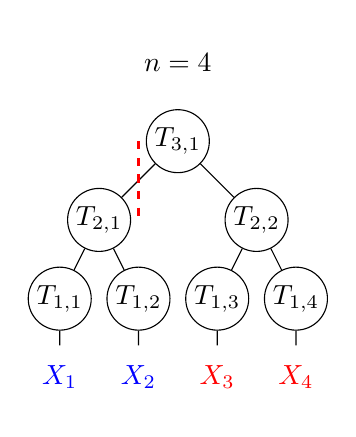
\begin{tikzpicture}[
                every node/.style={circle, draw, minimum size=8mm, inner sep=0pt},
                level distance=10mm,
                sibling distance=10mm,
                edge from parent/.style={draw},
                level 1/.style={sibling distance=20mm},
                level 2/.style={sibling distance=10mm}
            ]

            % Tree with 4 leaves
            \node[draw=none] at (1,0) {$n=4$};
            \node (t31) at (1, -1) {$T_{3,1}$} [grow=down]
            child {node (t21a) {$T_{2,1}$}
                child {node (t11c) {$T_{1,1}$}
                    child {node [draw=none] (x1) {$\textcolor{blue}{X_1}$}}}
                child {node (t13) {$T_{1,2}$}
                    child {node [draw=none] (x2) {$\textcolor{blue}{X_2}$}}}}
            child {node (t22) {$T_{2,2}$}
                child {node (t14) {$T_{1,3}$}
                    child {node [draw=none] (x3) {$\textcolor{red}{X_3}$}}}
                child {node (t15) {$T_{1,4}$}
                    child {node [draw=none] (x4) {$\textcolor{red}{X_4}$}}}};
            % \draw (t11c) -- ++(0,-0.7);
            % \draw (t13) -- ++(0,-0.7);
            % \draw (t14) -- ++(0,-0.7);
            % \draw (t15) -- ++(0,-0.7);

            % Min cut line
            \draw[dashed, red, thick, rounded corners] (0.5, -1) -- (0.5, -2);

            \end{tikzpicture}
            \caption{Cut in a binary tree tensor network.}
            \label{pic:cut_bttn}
        \end{figure}

        Thus,
        \[
            \operatorname{rank} [[T]]_{A,B} \leq cn^p \quad ,
        \]
        since all axes are per definition upper bounded by this function.

        Since $[[T]]_{A,B} \in \mathbb{R}^{|\Sigma|^{\frac{n}{2}} \times |\Sigma|^{\frac{n}{2}}}$, we see that for growing $n$ the matrix has not full rank and hence cannot take on arbitrary probability distributions.
    \end{proof}

    \subsection{Power-Law Behavior in PCBTTN}
    Now, the question is whether PCBTTN are still capable of modelling some probability distributions with power-law behavior. As it turns out, we can easily construct families of PCBTTN that satisfy either strong lower bound power-law behavior or upper bound power-law behavior.

    \begin{theorem}
        PCBTTN are capable of strong lower bound power-law behavior.
    \end{theorem}
    \begin{proof}
        Again, we show an explicit construction for the case $n = 4$ which can easily be generalized to arbitrary sizes. We aim to model the probability distribution
        \[
            p(X_1, \dots, X_n) =
            \begin{cases}
                \frac{1}{|\Sigma|} & \text{if } X_1 = \cdots = X_n \\
                0 & \text{otherwise}
            \end{cases}
            \quad .
        \]
        Clearly, this distributions implies a constant mutual information $I(X_i; X_j)$ for any pair $X_i, X_j$.

        So, how do we implement it? The graph of our network is depicted in figure~\ref{fig:binary_tree_tensor_network_n_equals_four_2}.
        \begin{figure}[h]
            \centering
            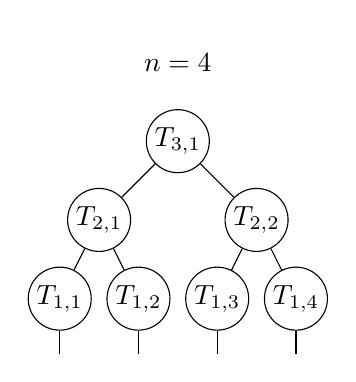
\begin{tikzpicture}[
                every node/.style={circle, draw, minimum size=8mm, inner sep=0pt},
                level distance=10mm,
                sibling distance=10mm,
                edge from parent/.style={draw},
                level 1/.style={sibling distance=20mm},
                level 2/.style={sibling distance=10mm}
            ]

            % Tree with 4 leaves
            \node[draw=none] at (1,0) {$n=4$};
            \node (t31) at (1, -1) {$T_{3,1}$} [grow=down]
            child {node (t21a) {$T_{2,1}$}
                child {node (t11c) {$T_{1,1}$}}
                child {node (t13) {$T_{1,2}$}}}
            child {node (t22) {$T_{2,2}$}
                child {node (t14) {$T_{1,3}$}}
                child {node (t15) {$T_{1,4}$}}};
            \draw (t11c) -- ++(0,-0.7);
            \draw (t13) -- ++(0,-0.7);
            \draw (t14) -- ++(0,-0.7);
            \draw (t15) -- ++(0,-0.7);

            \end{tikzpicture}
            \caption{Model structure of binary tree tensor networks for $n = 2^k = 4$.}
            \label{fig:binary_tree_tensor_network_n_equals_four_2}
        \end{figure}
        
        We start by initializing the bottom matrices $T_{1,k}$. We set them to identity matrices.

        Next, the tensors $T_{2,k}$ check for equality of their child tensor outputs and in case of equality return the one-hot encoded vector representing the shared random variable. Hence, they define the map
        \[
            T_{2,1}: \mathbb{R}^{|\Sigma|} \times \mathbb{R}^{|\Sigma|} \mapsto \mathbb{R}^{|\Sigma|}, (X_1, X_2) \mapsto
            \begin{cases}
                \bm{e}_i & \text{if } X_1 = X_2 = c_i \\
                \bm{0} & \text{otherwise}
            \end{cases}
            \quad ,
        \]
        where $c_i$ is the i-th character in $\Sigma$, and $\bm{e}_i$ is the i-th standard basis vector. $T_{2,2}$ is defined similarly.

        The matrix $T_{3,1}$ then does the final equality check of its child tensor outputs, i.e.
        \[
            T_{3,1}: \mathbb{R}^{|\Sigma|} \times \mathbb{R}^{|\Sigma|} \mapsto [0, 1], (X_1 = X_2, X_3 = X_4) \mapsto \bm{1}[X_1 = X_2 = X_3 = X_4] \cdot \frac{1}{|\Sigma|} \quad .
        \]
        Based on our construction, it is apparent that the tensor network implements the desired probability distributions $p$ with strong lower bound power-law behavior. Note that we only used a maximum axis size of $|\Sigma|$ which stays constant for growing $n$.
    \end{proof}

    \begin{theorem}
        PCBTTN are capable of upper bound power-law behavior.
    \end{theorem}
    \begin{proof}
        We aim to implement the uniform probability distribution
        \[
            p(X_1, \dots, X_n) \equiv \frac{1}{|\Sigma|^n} \quad .
        \]
        Of course, this implies a uniform probability distribution between any pair $X_i, X_j$ when marginalizing over the other variables. This implies that $I(X_i;X_j) = 0$, as they are independent.

        What we need to to is simply initialize the tensors $T_{1,k}$ to all-ones vectors, as it's a matrix with only one column so to speak.

        All the other tensors are then just scalars with the scalar value of $1$. The top most matrix in the network is also a scalar, but is set to $\frac{1}{|\Sigma|^n}$ instead.

        Apparently, this network implements the probability distribution $p$. Note that we only used axes sizes of $1$.
    \end{proof}

    These theorems were relatively straightforward. However, it remains to be determined whether we can combine upper bound and strong lower bound power-law behavior in a single PCBTTN, i.e. whether PCBTTN are capable of strong power-law behavior.
\end{document}